% Section content template for individual Educative lessons
% This file contains the actual content for a specific section
% Generated from Educative API section content

% Section: Memcached versus Redis
% Section ID: 5441771256938496
% Section Slug: memcached-versus-redis
% Generated: 2025-12-07T18:52:56.782951

\subsection{Introduction}\label{aZ2TKwPuDVp4vDxetsgtn}
\\
This lesson will discuss some of the widely adopted real-world implementations of a distributed cache. Our focus will be on two well-known open-source frameworks: Memcached and Redis. They 're highly scalable, highly performant, and robust caching tools. Both of these techniques follow the client-server model and achieve a latency of sub-millisecond. Let
's discuss each one of them and then compare their usefulness.

\subsection{Memcached}\label{TggiGXZeug4q4Yn5P4W4L}
\\
\textbf{Memcached} was introduced in 2003. It's a key-value store distributed cache designed to store objects very fast. Memcached stores data in the form of a key-value pair. Both the key and the value are strings. This means that any data that has been stored will have to be serialized(Serialization is the process of translating data into a format that can be transmitted or stored elsewhere. Later, reconstruction or deserialization of the data should be possible.). So, Memcached doesn't support and can't manipulate different data structures.
\\
Memcached has a client and server component, each of which is necessary to run the system. The system is designed in a way that half the logic is encompassed in the server, whereas the other half is in the client. However, each server follows the \textbf{shared-nothing architecture}. In this architecture, servers are unaware of each other, and there's no synchronization, data sharing, and communication between the servers.
\\
Due to the disconnected design, Memcached is able to achieve almost a deterministic query speed \protect\phantomsection\label{katex_inline_75gjssGxgsScR4N9UCJJb}{{{\(\text{(O(1))}\)}}} serving millions of keys per second using a high-end system. Therefore, Memcached offers a high throughput and low latency.

\begin{figure}[htbp]
 \centering
 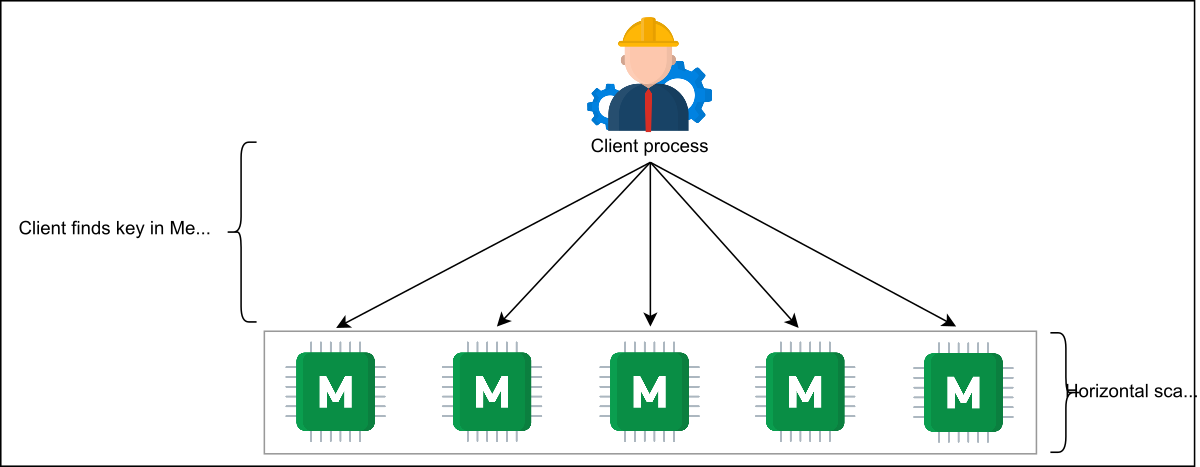
\includegraphics[width=0.5\textwidth]{Images/chapter_16/section_5441771256938496/6694696462319616.png}
 \caption{Design of a typical Memcached cluster}
\end{figure}

As evident from the design of a typical Memcached cluster, Memcached scales well horizontally. The client process is usually maintained with the service host that also interacts with the authoritative storage (back-end database).

\subsubsection{Facebook and Memcached}\label{NMr9-D3w8Qsh6UN7BMVQz}
\\
The data access pattern in Facebook requires frequent reads and updates because views are presented to the users on the fly instead of being generated ahead of time. Because Memcached is simple, it was an easy choice for the solution because Memcached started developing in 2003 whereas Facebook was developed in 2004. In fact, in some cases, Facebook and Memcached teams worked together to find solutions.\\

Redis was developed in 2009. So, using Redis wasn't a possibility at Facebook by then.

Some of the simple commands of Memcached include the following:

\begin{lstlisting}[language=JavaScript]
get <key_1> <key_2> <key_3> ...
set <key> <value> ...
delete <key>[<time>] ...
\end{lstlisting}

At Facebook, Memcached sits between the MySQL database and the web layer that uses roughly 28 TeraBytes of RAM spread across more than 800 servers (as of 2013(Facebook and Memcached - Tech Talk)). By an approximation of least recently used (LRU) eviction policy, Facebook is able to achieve a cache hit rate of 95\%.
\\
The following illustration shows the high-level design of caching architecture at Facebook. As we can see, out of a total of 50 million requests made by the web layer, only 2.5 million requests reach the persistence layer.

\begin{figure}[htbp]
 \centering
 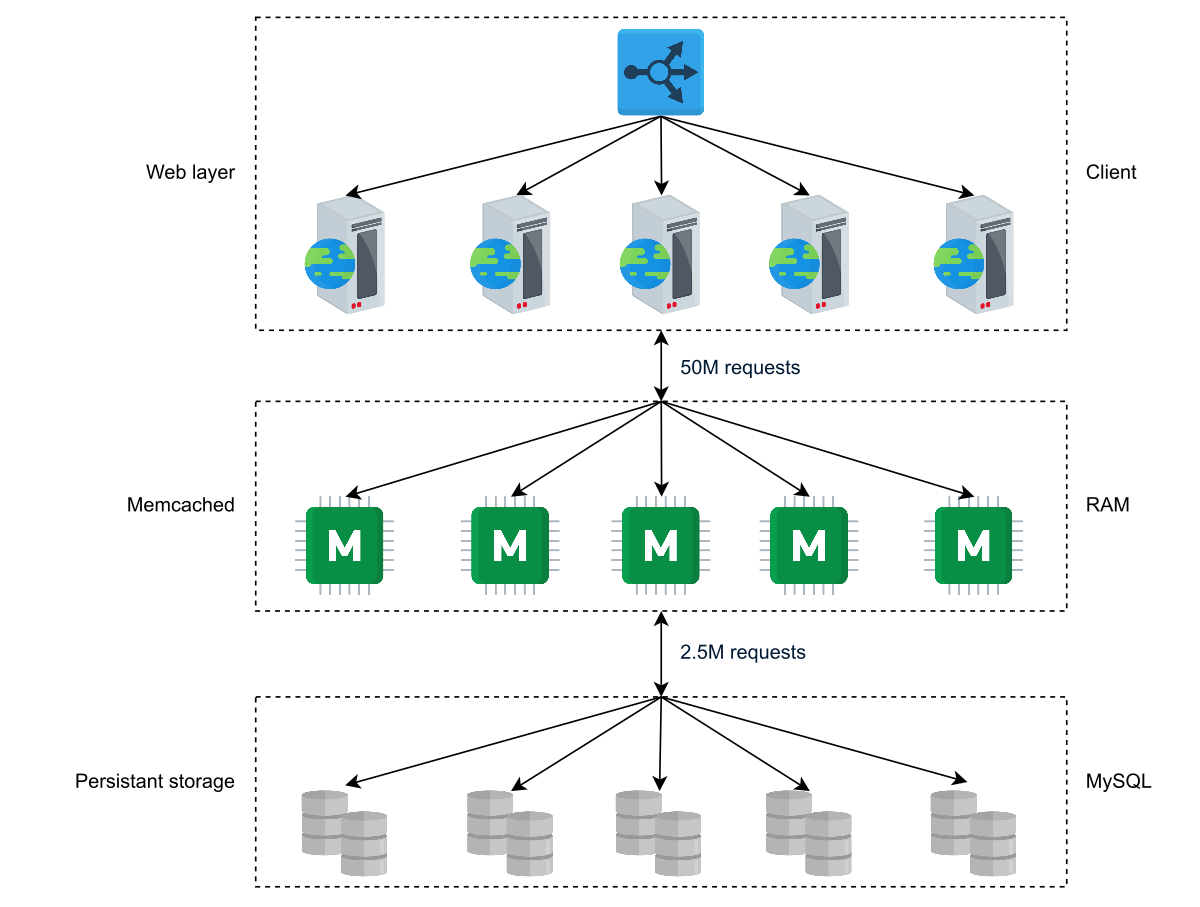
\includegraphics[width=0.5\textwidth]{Images/chapter_16/section_5441771256938496/5256469150957568.png}
 \caption{Facebook using a layer of Memcached sitting between persistence and web layer}
\end{figure}

\subsection{Redis}\label{uA6TlDUI4rXF0RzEXcwkC}
\\
\textbf{Redis} is a data structure store that can be used as a cache, database, and message broker. It offers rich features at the cost of additional complexity. It has the following features:

\begin{itemize}
\item
\protect\phantomsection\label{kAEt_ZQwfmN4PDtcAUflC}
\textbf{Data structure store}: Redis understands the different data structures it stores. We don't have to retrieve data structures from it, manipulate them, and then store them back. We can make in-house changes that save both time and effort.
\item
\protect\phantomsection\label{RyPKsCXzksHuwHqeJMvzq}
\textbf{Database}: It can persist all the in-memory blobs on the secondary storage.
\item
\protect\phantomsection\label{0kbNJQuSiNPOzRzbrXIXn}
\textbf{Message broker}: Asynchronous communication is a vital requirement in distributed systems. Redis can translate millions of messages per second from one component to another in a system.
\end{itemize}
\\
Redis provides a built-in replication mechanism, automatic failover, and different levels of persistence. Apart from that, Redis understands Memcached protocols, and therefore, solutions using Memcached can translate to Redis. A particularly good aspect of Redis is that it separates data access from cluster management. It decouples the control plane from the data plane. This results in increased reliability and performance. Finally , Redis doesn't provide strong consistency due to the use of asynchronous replication.

\begin{figure}[htbp]
 \centering
 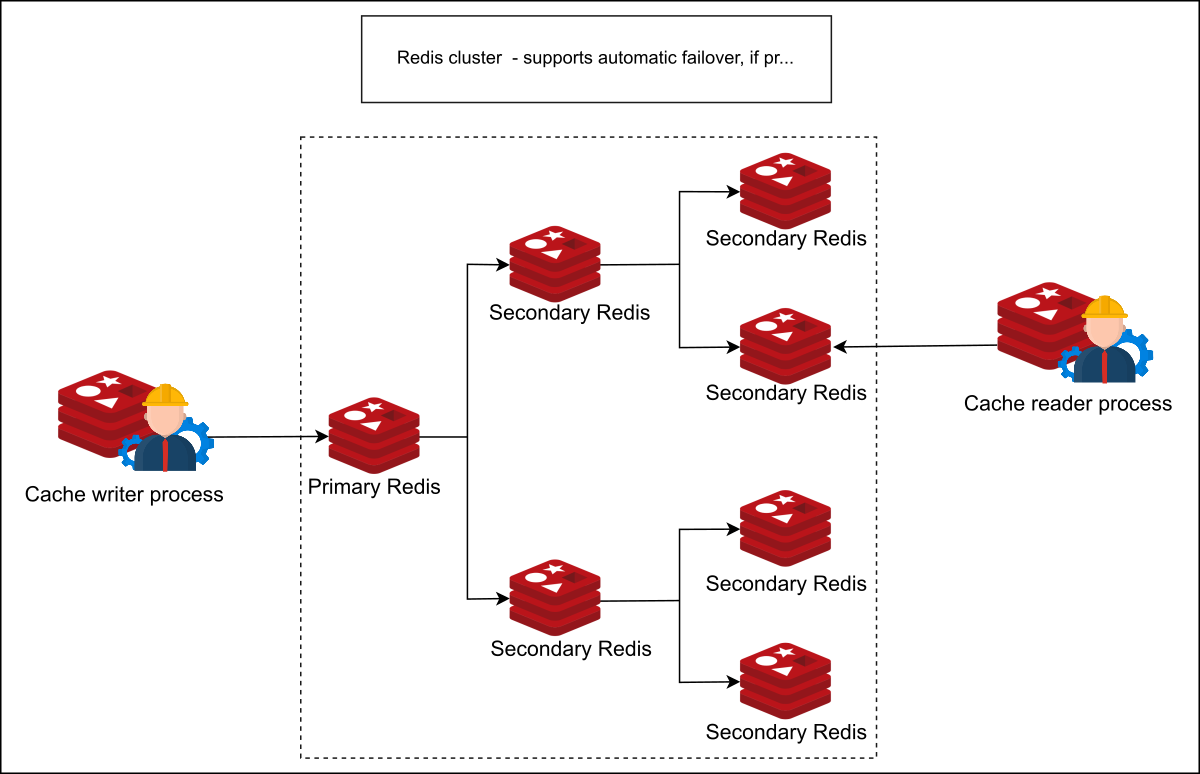
\includegraphics[width=0.5\textwidth]{Images/chapter_16/section_5441771256938496/5678630076416000.png}
 \caption{Redis structure supporting automatic failover using redundant secondary replicas}
\end{figure}

\subsubsection{Redis cluster}\label{SfmwfwwqELd1Oyo3B0S10}
\\
Redis has built-in cluster support that provides high availability. This is called Redis Sentinel. A cluster has one or more Redis databases that are queried using multithreaded proxies. Redis clusters perform automatic sharding where each shard has primary and secondary nodes. However, the number of shards in a database or node is configurable to meet the expectations and requirements of an application.\\
\strut \\
Each Redis cluster is maintained by a cluster manager whose job is to detect failures and perform automatic failovers. The management layer consists of monitoring and configuration software components.\\
\strut \\

\begin{figure}[htbp]
 \centering
 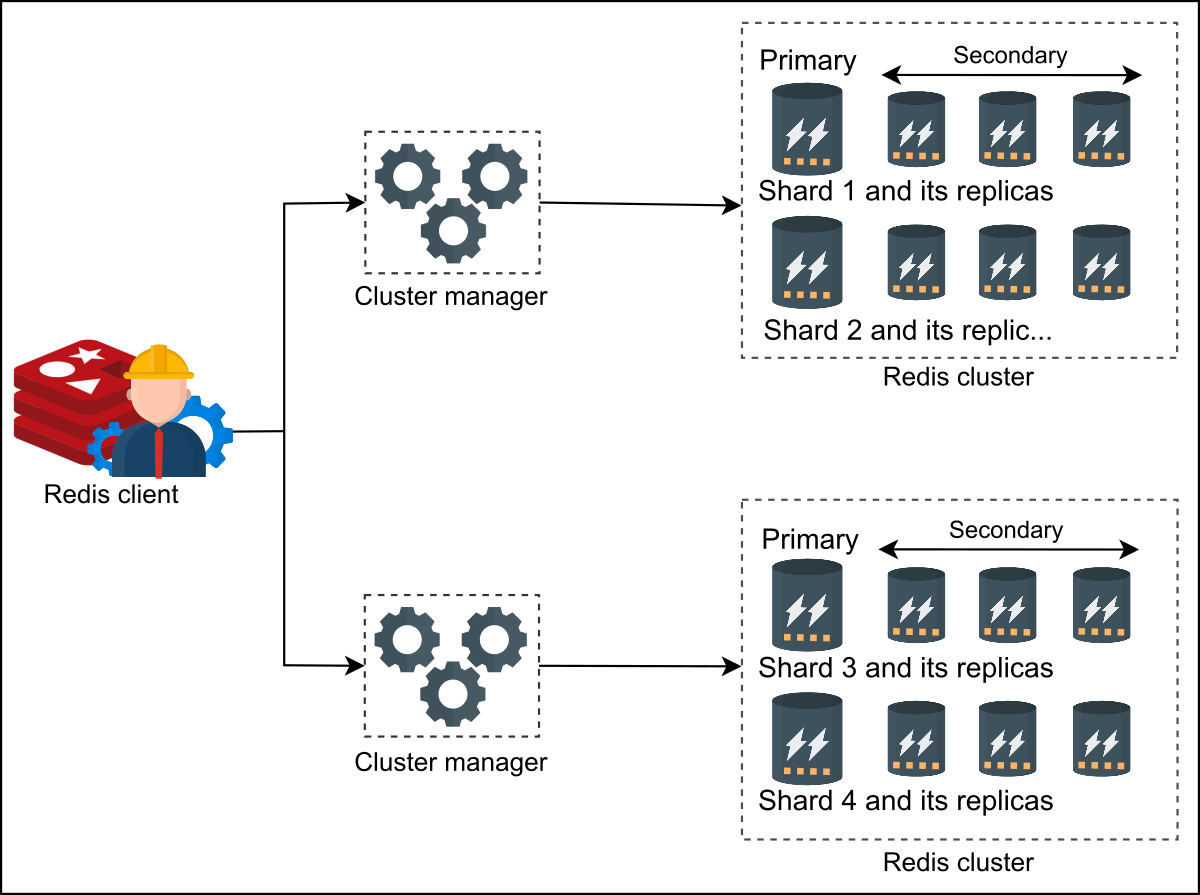
\includegraphics[width=0.3\textwidth]{Images/chapter_16/section_5441771256938496/5864162328838144.png}
 \caption{Architecture of Redis clusters}
\end{figure}

\subsubsection{Pipelining in Redis}\label{tW3GQ1wazaR-3Lulg3xfA}
\\
Since Redis uses a client-server model, each request blocks the client until the server receives the result. A Redis client looking to send subsequent requests will have to wait for the server to respond to the first request. So , the overall latency will be higher.
\\
Redis uses \textbf{pipelining} to speed up the process. \textbf{Pipelining} is the process of combining multiple requests from the client side without waiting for a response from the server. As a result, it reduces the number of RTT(The round-trip-time (RTT) is the latency for a request to travel from the client to the server and back.) spans for multiple requests.

\begin{figure}[htbp]
 \centering
 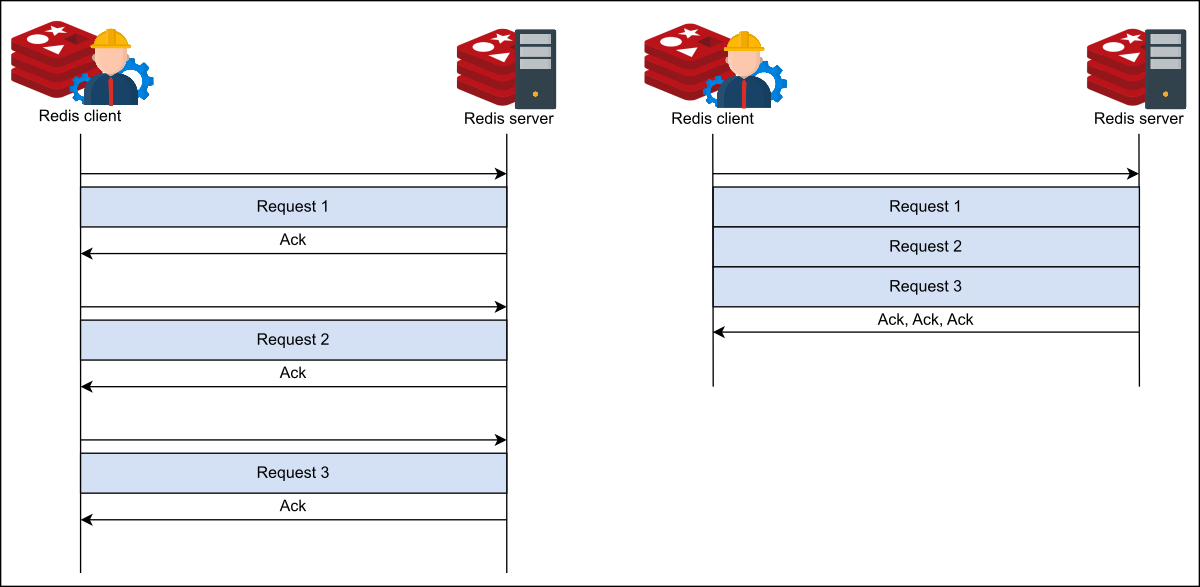
\includegraphics[width=0.3\textwidth]{Images/chapter_16/section_5441771256938496/6728524161613824.png}
 \caption{Redis client-server communication without pipelining versus Redis client-server communication with pipelining}
\end{figure}

The process of pipelining reduces the latency through RTT and the time to do socket level I/O. Also , mode switching through system calls in the operating system is an expensive operation that's reduced significantly via pipelining. Pipelining the commands from the client side has no impact on how the server processes these requests.
\\
For example, two requests pipelined by the client reach the server, and the server can't entertain the second. The server provides a result for the first and returns an error for the second. The client is independent in batching similar commands together to achieve maximum throughput.
\begin{quote}
\textbf{Note:} Pipelining improves the latency to a minimum of five folds if both the client and server are on the same machine. The request is sent on a loopback address (\texttt{127.0.0.1}). The true power of pipelining is highlighted in systems where requests are sent to distant machines.
\end{quote}
\subsection{Memcached versus Redis}\label{X49kIBN1bZWQZ5_BeJLAN}
\\
Even though Memcached and Redis both belong to the NoSQL family, there are subtle aspects that set them apart:

\begin{itemize}
\item
\protect\phantomsection\label{B97bPo8ZN2E-5pMfkIIfY}
\textbf{Simplicity:} Memcached is simple, but it leaves most of the effort for managing clusters left to the developers of the cluster. This, however, means finer control using Memcached. Redis, on the other hand, automates most of the scalability and data division tasks.
\item
\protect\phantomsection\label{D2uaHCtz2gCiPNnHBmg_U}
\textbf{Persistence:} Redis provides persistence by properties like append only file (AOF) and Redis database (RDB) snapshot. There's no persistence support in Memcached. But this limitation can be catered to by using third-party tools(For example, libmemcached-tools).
\item
\protect\phantomsection\label{c1UNgWr94140SpnebGB3J}
\textbf{Data types}: Memcached stores objects in the form of key-value pairs that are both strings, whereas Redis supports strings, sorted sets, hash maps, bitmaps, and hyper logs. However, the maximum key or value size is configurable.
\item
\protect\phantomsection\label{mdt10_h6IbsjO7moqVqNx}
\textbf{Memory usage:} Both tools allow us to set a maximum memory size for caching. Memcached uses the slab allocation method for reducing fragmentation. However, when we update the existing entries' size or store many small objects, there may be a wastage of memory. Nonetheless, there are configuration workarounds to resolve such issues.
\item
\protect\phantomsection\label{InWvd2nFrYz4F1Nc1VNrE}
\textbf{Multithreading:} Redis runs as a single process using one core, whereas Memcached can efficiently use multicore systems with multithreading technology. We could argue that Redis was designed to be a single-threaded process that reduces the complexity of multithreaded systems. Nonetheless, multiple Redis processes can be executed for concurrency. At the same time, Redis has improved over the years by tweaking its performance. Therefore, Redis can store small data items efficiently. Memcached can be the right choice for file sizes above 100 K.
\item
\protect\phantomsection\label{jBeJI4ILU8dQSdOcdzcjU}
\textbf{Replication:} As stated before, Redis automates the replication process via few commands, whereas replication in Memcached is again subject to the usage of third-party tools. Architecturally, Memcached can scale well horizontally due to its simplicity. Redis provides scalability through clustering that's considerably complex.
\end{itemize}
\\
The table below summarizes some of the main differences and common features between Memcached and Redis:

\textbf{Features Offered by Memcached and Redis}

\begin{table}[htbp]
\centering
\small
\adjustbox{max width=\textwidth}{
\begin{tabular}{|p{0.317\textwidth}|p{0.317\textwidth}|p{0.317\textwidth}|}
\hline
\textbf{Feature} & \textbf{Memcached} & \textbf{Redis} \\
\hline
\hline
Low latency & Yes & Yes \\
\hline
Persistence & Possible via third-party tools & Multiple options \\
\hline
Multilanguage support & Yes & Yes \\
\hline
Data sharding & Possible via third-party tools & Built-in solution \\
\hline
Ease of use & Yes & Yes \\
\hline
Multithreading support & Yes & No \\
\hline
Support for data structure & Objects & Multiple data structures \\
\hline
Support for transaction & No & Yes \\
\hline
Eviction policy & LRU & Multiple algorithms \\
\hline
Lua scripting support & No & Yes \\
\hline
Geospatial support & No & Yes \\
\hline
\end{tabular}
}
\caption{Features Offered by Memcached and Redis}
\end{table}

To summarize, Memcached is preferred for smaller, simpler read-heavy systems, whereas Redis is useful for systems that are complex and are both read- and write-heavy.

\begin{quote}
\textbf{Quiz:}
\textbf{Question 1:} Based on the implementation details, which of the two frameworks

(Memcached or Redis) has a striking similarity with the distributed cache that we designed in the previous lesson?
\textbf{Answer:} The answer is Memcached. The reasons are as follows: Client software chooses which cache server to use with a hashing algorithm. Server software stores the values against each key using an internal hash table. Least recently used (LRU) is used as the eviction policy.

There's no communication between different cache servers.
\textbf{Question 2:} Why do third-party tools exist for persisting Memcached data?
\textbf{Answer:} It's because a lot of data is read and written to cache servers, and they may occasionally crash for whatever reason. After restarting,

building a cache from scratch can take up to hours in specific scenarios, and that ultimately reduces system performance. Therefore, cache data may be persisted to disk to be loaded on a restart.
\textbf{Question 3:} What is the advantage of storing different data structures as compared to strings only?
\textbf{Answer:} The main advantage is that Redis can modify data in place without wasting network bandwidth by downloading and uploading. It saves network bandwidth, but it also saves time and effort by avoiding the serialization and deserialization of data.
\end{quote}

\subsection{Conclusion}\label{BywEvPf3LPnjzWij7-aD6}
\\
\hfill\break
It's impossible to imagine high-speed large-scale solutions without the use of a caching system. In this chapter, we covered the need for a caching system and its fundamental details, and we orchestrated a basic distributed cache system. We also familiarized ourselves with the design and features of two of the most well-known caching frameworks.

% End of section content